% bitmaps.tex
%
% written 2022 by Werner Lemberg <wl@gnu.org>


% This file contains graphics used for the 'FreeType Glyph Conventions'
% tutorial, part 7, 'FreeType Bitmaps'.


% Here is one possibility to convert this LaTeX file to both PNG and SVG
% formats.
%
%   xelatex bitmaps.tex
%
%   pdftoppm -png -f 1 -l 4 -r 120 bitmaps.pdf bitmaps
%   optipng bitmaps-*.png
%
%   for i in 1 2 3 4; do
%     pdf2svg bitmaps.pdf bitmaps-$i.svg $i
%   done


\documentclass[tikz, border=3mm]{standalone}

\usepackage{libertinus}
% We want bold italic in math mode (via the `\symbfit` macro).
\usepackage{unicode-math}

\usetikzlibrary{
  calc
}


% Node styles.
\tikzset{
  % Shared values that are assigned to different keys in the styles below.
  % Taken from
  % https://tex.stackexchange.com/questions/660910/tikz-how-to-set-one-style-to-values-of-another-style
  globals/grid line width/.initial=0.5pt,
  globals/grid size/.initial=6mm,
%
  % For main curves.
  line/.style={
    line width=1pt},
%
  % For grid lines.
  grid line/.style={
    step=\pgfkeysvalueof{/tikz/globals/grid size},
    line width=\pgfkeysvalueof{/tikz/globals/grid line width},
    dash pattern=on 0.5mm off 0.5mm,
    dash phase=0.25mm},
%
  % For horizontal 'grid stripes'.
  grid stripe/.style={
    ystep=\pgfkeysvalueof{/tikz/globals/grid size},
    line width=\pgfkeysvalueof{/tikz/globals/grid line width},
  },
%
  % For thick curves with one arrow.
  axis/.style={
    line,
    -latex,
    line cap=rect},
%
  % For pixel centers.  This is essentially a transparent pixel box with a
  % small circle at its center.
  pixel center/.style={
    draw=none,
    minimum size=\pgfkeysvalueof{/tikz/globals/grid size},
    inner sep=0pt,
    outer sep=0pt,
    anchor=south west,
    append after command={%
      \pgfextra{%
        \node[circle,
              fill,
              minimum size=1pt,
              inner sep=0pt] at (\tikzlastnode.center) {};}}},
%
  % For pixels.  We both fill and draw to cover the grid lines.
  pixel/.style={
    line width=\pgfkeysvalueof{/tikz/globals/grid line width},
    draw,
    minimum size=\pgfkeysvalueof{/tikz/globals/grid size},
    fill,
    inner sep=0pt,
    outer sep=0pt,
    anchor=south west},
%
  % For squares.
  square/.style={
    fill,
    minimum size=4pt,
    inner sep=0pt,
    outer sep=0pt},
%
  % For descriptions.
  description/.style={
    label position=above left,
    font=\bfseries,
    align=right,
    yshift=-1ex},
%
  % For display of a large glyph.
  glyph/.style={
    font={\fontsize{80pt}{0pt}\selectfont},
    anchor=base west}
}


%%%%%%%%%%%%%%%%%%%%%%%%%%%%%%%%%%%%%%%%%%%%%%%%%%%%%%%%%%%%%%%%%%%%%%%%%%%%%

\begin{document}

% A bitmap and its vectorial grid.

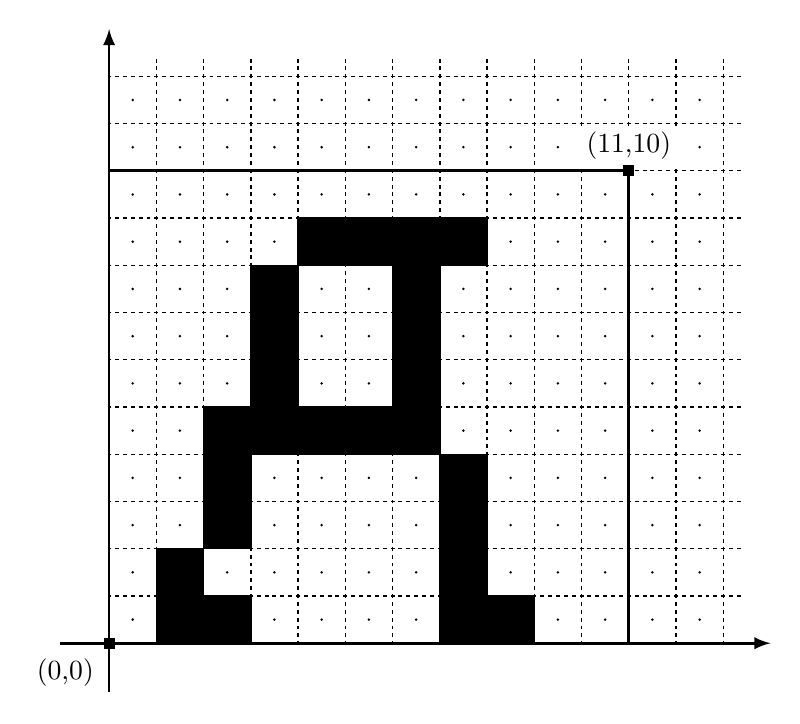
\begin{tikzpicture}
  \def\numX{11}
  \def\numY{10}

  \draw[grid line]
    % Save grid size in global macro.
    \pgfextra{\xdef\gridSize{\pgfkeysvalueof{/tikz/globals/grid size}}}
    (0,0) grid ($ ({(\numX+2)*\gridSize},
                   {(\numY+2)*\gridSize}) + (0.25,0.25) $);

  \draw[axis] (-\gridSize,0) -- ({(\numX+3)*\gridSize},0);
  \draw[axis] (0,-\gridSize) -- (0,{(\numY+3)*\gridSize});

  % Based on
  % https://tex.stackexchange.com/questions/157080/can-tikz-create-pixel-art-images
  \def\pixels{
    { , , , , , , , , , , , , },
    { , , , , , , , , , , , , },
    { , , , , , , , , , , , , },
    { , , , ,X,X,X,X, , , , , },
    { , , ,X, , ,X, , , , , , },
    { , , ,X, , ,X, , , , , , },
    { , , ,X, , ,X, , , , , , },
    { , ,X,X,X,X,X, , , , , , },
    { , ,X, , , , ,X, , , , , },
    { , ,X, , , , ,X, , , , , },
    { ,X, , , , , ,X, , , , , },
    { ,X,X, , , , ,X,X, , , , }}

  \foreach \line [count=\yy,
                  evaluate=\yy as \y using int(\numY+2-\yy)] in \pixels
    {\foreach \pix [count=\xx,
                    evaluate=\xx as \x using int(\xx-1)] in \line
      {\ifx\pix\empty
         \node[pixel center] at ({\x*\gridSize},{\y*\gridSize}) {};
       \else
         \node[pixel] at ({\x*\gridSize},{\y*\gridSize}) {};
       \fi}}

  \coordinate (ul) at ({\numX*\gridSize},{\numY*\gridSize});

  \draw[line] (0,0) rectangle (ul);
  \node[square,
        label={below left:(0,0)}] at (0,0) {};
  \node[square,
        label={[fill=white,
                inner ysep=2pt]above:(\numX,\numY)}] at (ul) {};
\end{tikzpicture}


% Positive pitch outline.

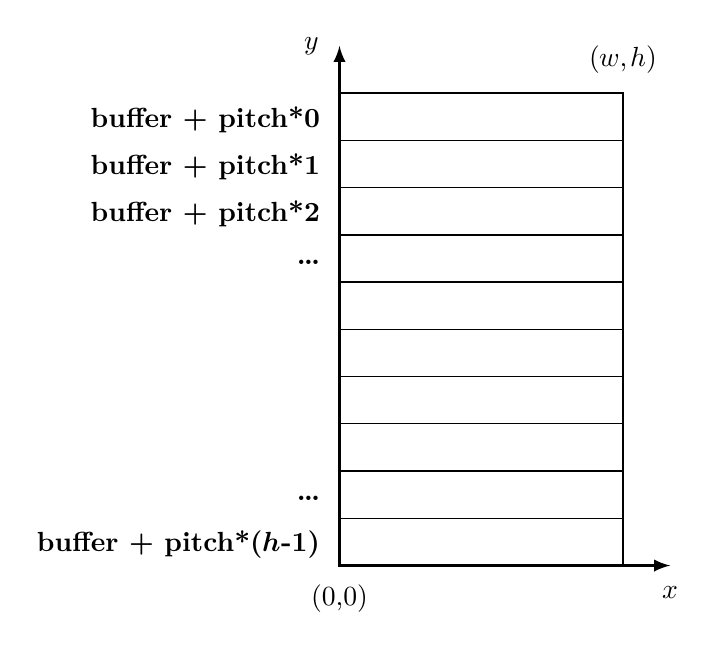
\begin{tikzpicture}
  \def\w{6}
  \def\h{10}

  \draw[line cap=rect]
    \pgfextra{\xdef\gridSize{\pgfkeysvalueof{/tikz/globals/grid size}}}
    [grid stripe,
     xstep={\w*\gridSize}] (0,0) grid ({\w*\gridSize},{\h*\gridSize});

  \draw[axis] (0,0) -- ({(\w+1)*\gridSize},0)
    node[label=below:$x$] {};
  \draw[axis] (0,0) -- (0,{(\h+1)*\gridSize})
    node[label=left:$y$] {};

  \node[label={below:(0,0)}]
    at (0,0) {};
  \node[label={above:($w$,\kern0.1em $h$)}]
    at ({\w*\gridSize},{\h*\gridSize}) {};

  \node[label={[description]buffer + pitch*0}] at (0,{(\h-1)*\gridSize}) {};
  \node[label={[description]buffer + pitch*1}] at (0,{(\h-2)*\gridSize}) {};
  \node[label={[description]buffer + pitch*2}] at (0,{(\h-3)*\gridSize}) {};
  \node[label={[description]\strut\dots}]
    at (0,{(\h-4)*\gridSize}) {};

  \node[label={[description]\strut\dots}]
    at (0,{1*\gridSize}) {};
  \node[label={[description]buffer + pitch*($\symbfit{h}$-1)}]
    at (0,{(0*\gridSize}) {};
\end{tikzpicture}


% Negative pitch outline.

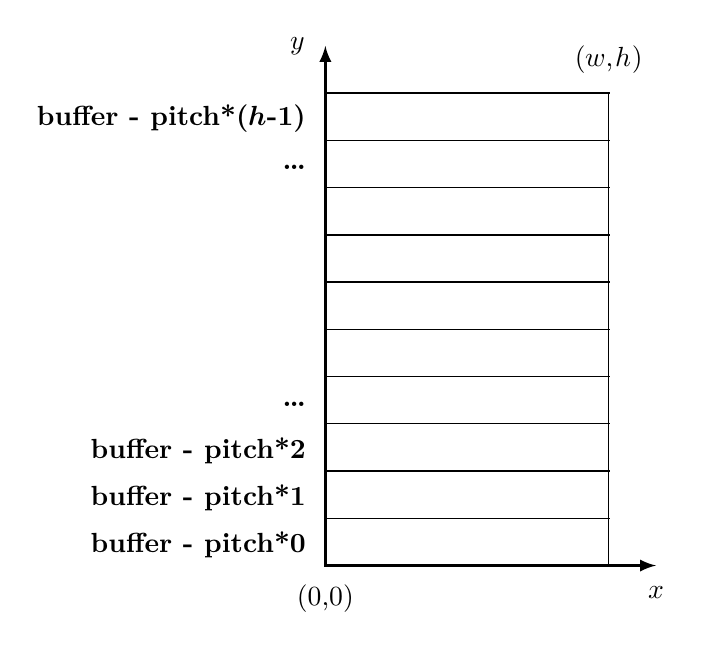
\begin{tikzpicture}
  \def\w{6}
  \def\h{10}

  \draw[line cap=rect]
    \pgfextra{\xdef\gridSize{\pgfkeysvalueof{/tikz/globals/grid size}}}
    [grid stripe,
     xstep={\w*\gridSize}] (0,0) grid ({\w*\gridSize},{\h*\gridSize});

  \draw[axis] (0,0) -- ({(\w+1)*\gridSize},0)
    node[label=below:$x$] {};
  \draw[axis] (0,0) -- (0,{(\h+1)*\gridSize})
    node[label=left:$y$] {};

  \node[label={below:(0,0)}]
    at (0,0) {};
  \node[label={above:($w$,\kern0.1em $h$)}]
    at ({\w*\gridSize},{\h*\gridSize}) {};

  \node[label={[description]buffer - pitch*0}] at (0,{0*\gridSize}) {};
  \node[label={[description]buffer - pitch*1}] at (0,{1*\gridSize}) {};
  \node[label={[description]buffer - pitch*2}] at (0,{2*\gridSize}) {};
  \node[label={[description]\strut\dots}]
    at (0,{3*\gridSize}) {};

  \node[label={[description]\strut\dots}]
    at (0,{(\h-2)*\gridSize}) {};
  \node[label={[description]buffer - pitch*($\symbfit{h}$-1)}]
    at (0,{(\h-1)*\gridSize}) {};
\end{tikzpicture}


% Demonstrate incorrect clipping.

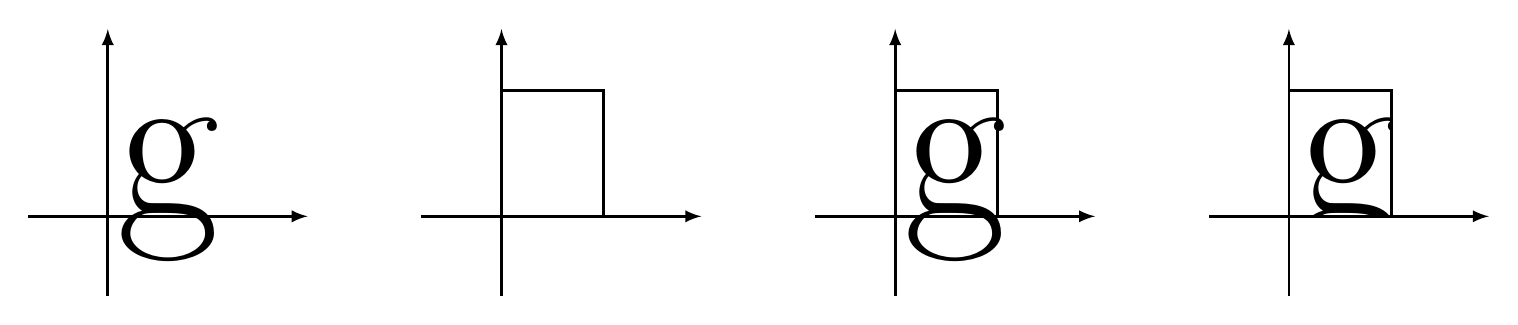
\begin{tikzpicture}
  \def\glyph{\node[glyph] (glyph) at (0,0) {g};}
  \def\xAxis{\draw[axis] (-1,0) -- ({\glyphWidth+1cm},0);}
  \def\yAxis{\draw[axis] (0,-1) -- ($(glyph.north -| 0,1) + (0,1)$);}
  \def\rect{(1.3,1.6)}
  \def\rectangle{\draw[line] (0,0) rectangle \rect;}

  \glyph

  % A dummy path to define `\glypWidth` macro.
  \path
    let \p{width}=($ (glyph.east)-(glyph.west) $)
    in  \pgfextra{\xdef\glyphWidth{\x{width}}} (0,0);

  \xAxis
  \yAxis

  \tikzset{shift={(5,0)}}
  \rectangle
  \xAxis
  \yAxis

  \tikzset{shift={(5,0)}}
  \glyph
  \rectangle
  \xAxis
  \yAxis

  \tikzset{shift={(5,0)}}
  \begin{scope}
    \clip (0,0) rectangle \rect;
    \glyph
  \end{scope}
  \rectangle
  \xAxis
  \yAxis
\end{tikzpicture}

\end{document}
